\section{Deriving rate constants}
\label{subsec:rate-constants}

In the experiment, the parent ion \CD and He$_n$CD$^+$ complexes counts are
monitored as a function of trap time (in the following, it will be referred to
as \qt{kinetics scan}) where all ions are monitored for a duration of up to 6
s, with 4-5 iterations per data point, as shown in Figure
\ref{fig:fit:rate-constants}. The coupled ordinary differential (ODE) rate
equations, as discussed in section \ref{subsec:rate-equations} and
\ref{subsec:rate-loss-channels}, are solved using the implicit Runge-Kutta
method of the Radau IIA family of order 5 \cite{hairer_implementation_1996},
and the solution is numerically fitted to the measured data using the
Levenberg-Marquardt algorithm also known as damped least-squares (DLS) method
(as shown as solid lines in Figure \ref{fig:fit:rate-constants}) to derive the
rates [\pers] $R_e$ and $R_{CID}$. These computations are carried out using the
SciPy library \cite{virtanen_scipy_2020}. The corresponding rate coefficients
are derived from the rates as described in equations
\ref{eqn:rate-theory:R*-simplified} and \ref{eqn:rate:rcid}.

\begin{figure}[!htb]

    \centering

    \begin{subfigure}[b]{0.49\textwidth}
        \centering
        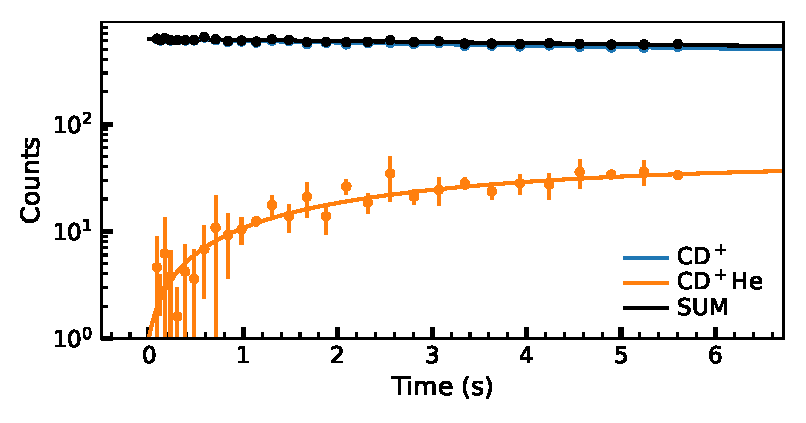
\includegraphics[width=1\textwidth]{figures/measurements/kinetics/off_kinetics_1.16_2e+14.pdf}
        \caption{}
        
    \end{subfigure}
    \hfill
    \begin{subfigure}[b]{0.49\textwidth}
        \centering
        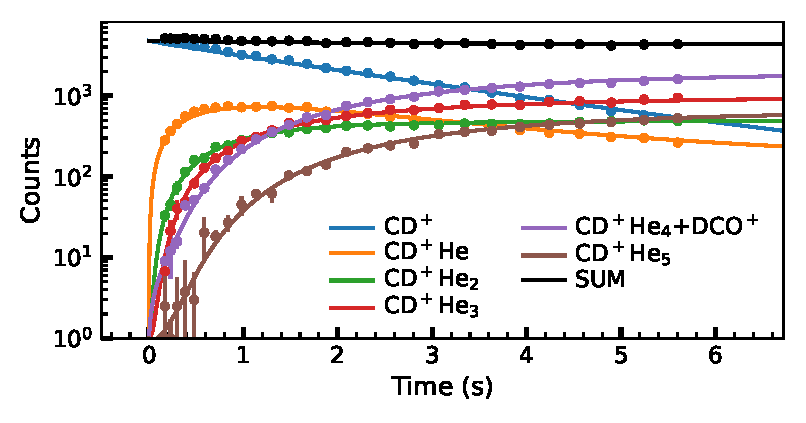
\includegraphics[width=1\textwidth]{figures/measurements/kinetics/off_kinetics_6.04_25e+14.pdf}
        \caption{}
        
    \end{subfigure}
    
    \caption{(a) and (b) show the counts of primary and complex ions monitored as a function of trap time at number densities of $ 1.16(2)\cdot10^{14}$~cm$^{-3}$ and  $6.0(2)\cdot10^{14}$~cm$^{-3}$, respectively, and at a trap temperature of 4.8(3) K. The circle marker and the solid line represent measured and numerically fitted data, respectively.}
    \label{fig:fit:rate-constants}

\end{figure}
\begin{figure}[!htb]
    \centering
    \begin{subfigure}[b]{0.49\textwidth}
        \centering
        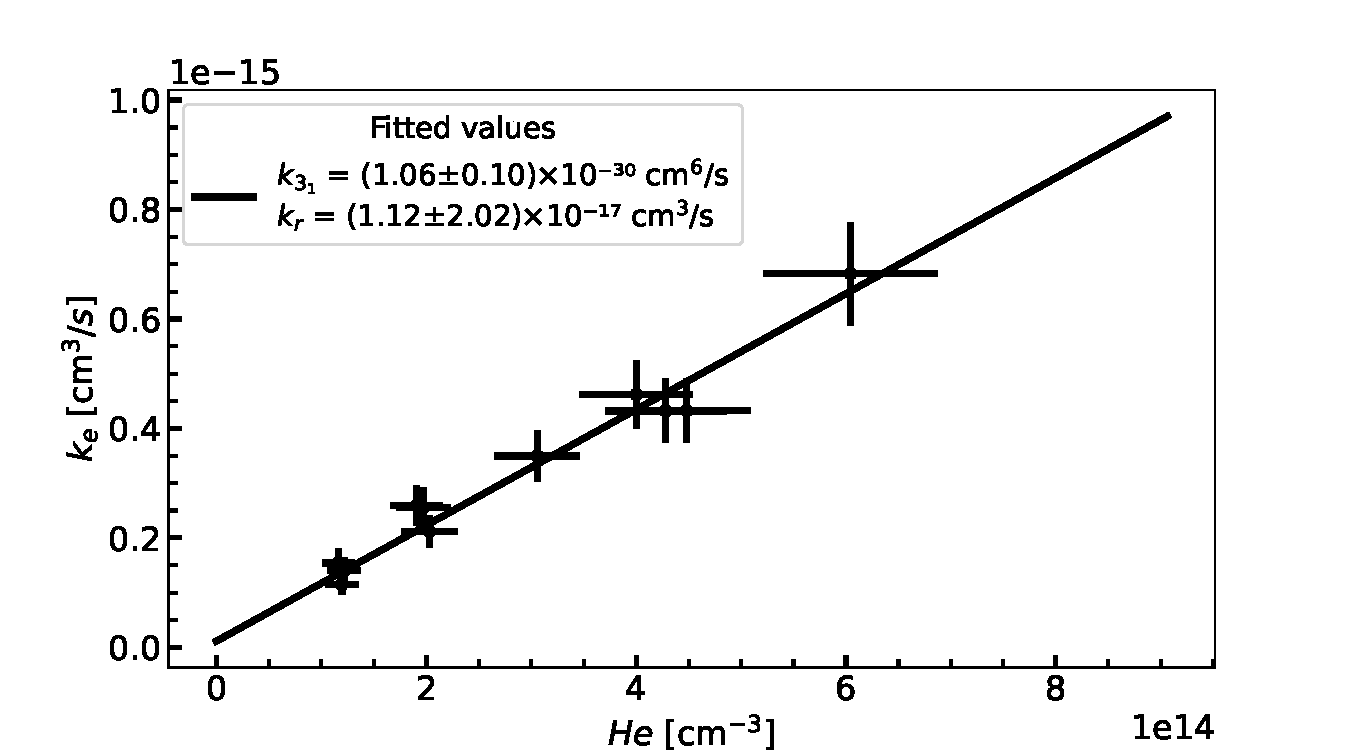
\includegraphics[width=1\textwidth]{figures/measurements/kinetics/functionOf_nHe/off_4.8K_k31_effective_rate_constants.pdf}
        
        \caption{}
        \label{fig:off:effective-rate-constants}
    \end{subfigure}
    \hfill
    \begin{subfigure}[b]{0.49\textwidth}
        \centering
        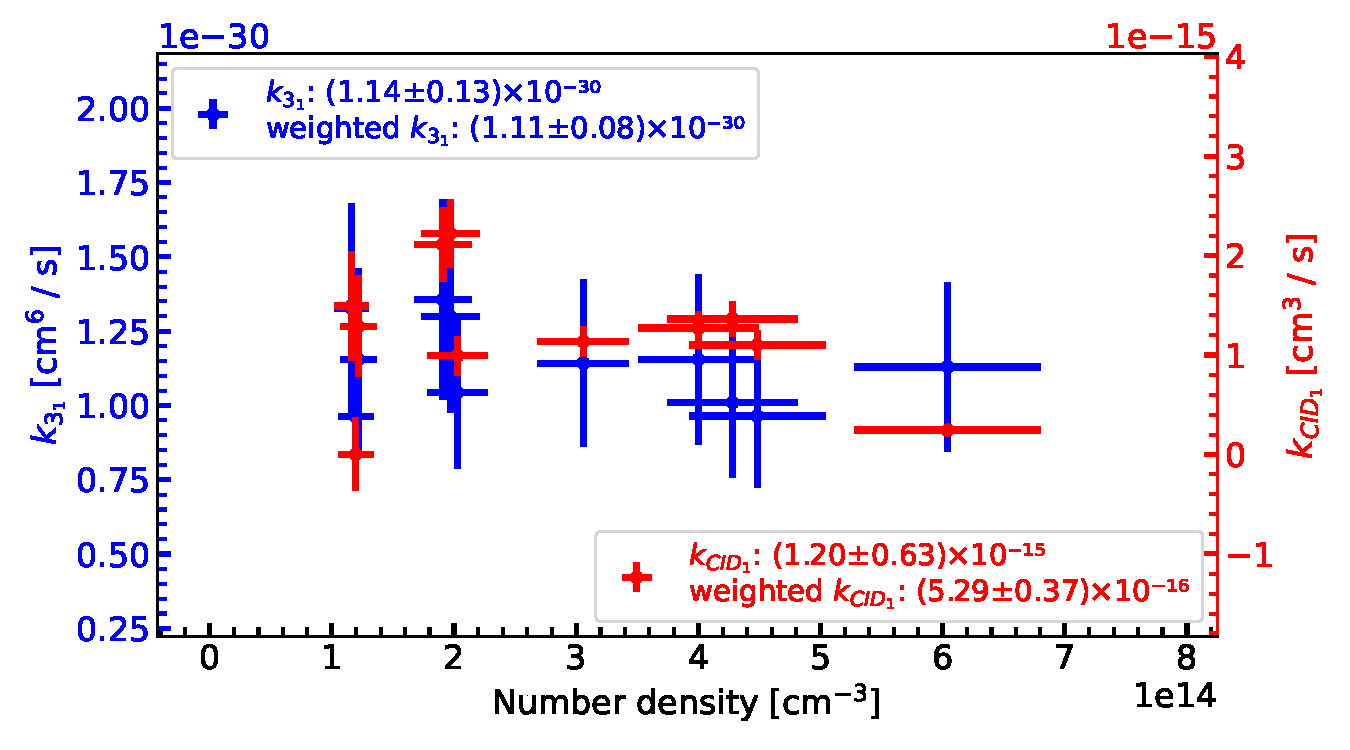
\includegraphics[width=1\textwidth]{figures/measurements/kinetics/functionOf_nHe/off_4.8K_k3_kCID_1_as_functionOfnHe.pdf}
        \caption{}
        \label{fig:off:rate-constants}
    \end{subfigure}
    
    \caption{The effective binary rate constant ($k_e$), the ternary association (\textcolor{blue}{$k_{3_1}$}) and collision-induced dissociation (\textcolor{red}{$k_{CID_1}$}) rate constants are plotted as a function of helium number density. (a) The effective binary rate constant ($k_e$) is plotted as a function of number density to derive $k_{3_1}$ (ternary association) and $k_r$ (radiative) rate constants. The solid line indicates the linear fit where the slope and intercept correspond to $k_3$ and $k_r$, respectively. (b) shows the $k_{3_1}$ as a function of number density under $k_3[He] \gg k_r$ assumption (see text). The weighted mean values are shown in the legend box.}

\end{figure}


Figure \ref{fig:off:effective-rate-constants} shows exemplary the derived
effective binary rate constant $k_e$ plotted against the Helium number density
    [He] to determine the ternary association rate constant ($k_3$) and radiative
rate ($k_r$) using Eq. \ref{eqn:rate-theory:k*-simplified} at 4.8(3) K
temperature. The radiative rate, $k_r=1.2(1.9) \cdot 10^{-17}$\pers\ could not be
determined, and the derived error margin can be viewed as an upper limit to
this value. Thus, one can simplify the equation
\ref{eqn:rate-theory:R*-simplified} such that $k_3[He] >> k_r$, then:

\begin{equation}
    R_e = k_e[He] = k_3[He]^2
    \label{eqn:rate-theory:k*-further-simplified}
\end{equation}

\begin{threeparttable}[!htb]
    \centering
    \caption{Comparing derived $k_{3_n}$ rate coefficients [in cm$^6$s$^{-1}$] in this work to previous results from \citet{Brunken2017}}
     \begin{tabular}{ccccccc}
        \hline\\
        & T$_{trap} [K]$ & T$_{ion} [K]$& $k_{3_1}$ &  $k_{3_2}$ & $k_{3_3}$ & $k_{3_4}$ \\
        &&& $\times 10^{-30}$ & $\times 10^{-30}$ & $\times 10^{-30}$ & $\times 10^{-30}$\\
        \\\hline\hline\\
        this work & 4.8(3) & 15(3) & $1.1(1)$ & $3.6(4)$ & $13(2)$ & $10(1)$ \\
        Ref \cite{Brunken2017} & 5 & 12(1) & $1.2(1)$ & $3.7(3)$ & $13(2)$ & $19(2)$ \\
        \\\hline\hline\\
    \end{tabular}
    \label{tab:k3:rate-constants}
\end{threeparttable}

\begin{threeparttable}[!htb]
    \centering
    \caption{Comparing derived  $k_{CID_n}$ rate constants [in cm$^3$s$^{-1}$] in this work to previous results from \citet{Brunken2017}}
    \begin{tabular}{ccccccc}
        \hline\\
        & T$_{trap} [K]$ & T$_{ion} [K]$& $k_{CID_1}$ &  $k_{CID_2}$ & $k_{CID_3}$ & $k_{CID_4}$ \\
        &&& $\times 10^{-16}$ & $\times 10^{-15}$ & $\times 10^{-15}$ & $\times 10^{-15}$\\
        \\\hline\hline\\
        this work & 4.8(3) &  15(3) & $5.2(1.5)$ & $1.2(2)$ & $4.3(5)$ & $2.4(6)$ \\
        Ref \cite{Brunken2017} & 5 & 12(1) & $9(2)$ & $1.9(2)$ & $6.5(9)$ & $11(3)$ \\
        \\\hline\hline\\
    \end{tabular}
    \label{tab:kCID:rate-constants}
\end{threeparttable}
\begin{figure}[!htb]

    \centering

    \begin{subfigure}[b]{0.49\textwidth}
        \centering
        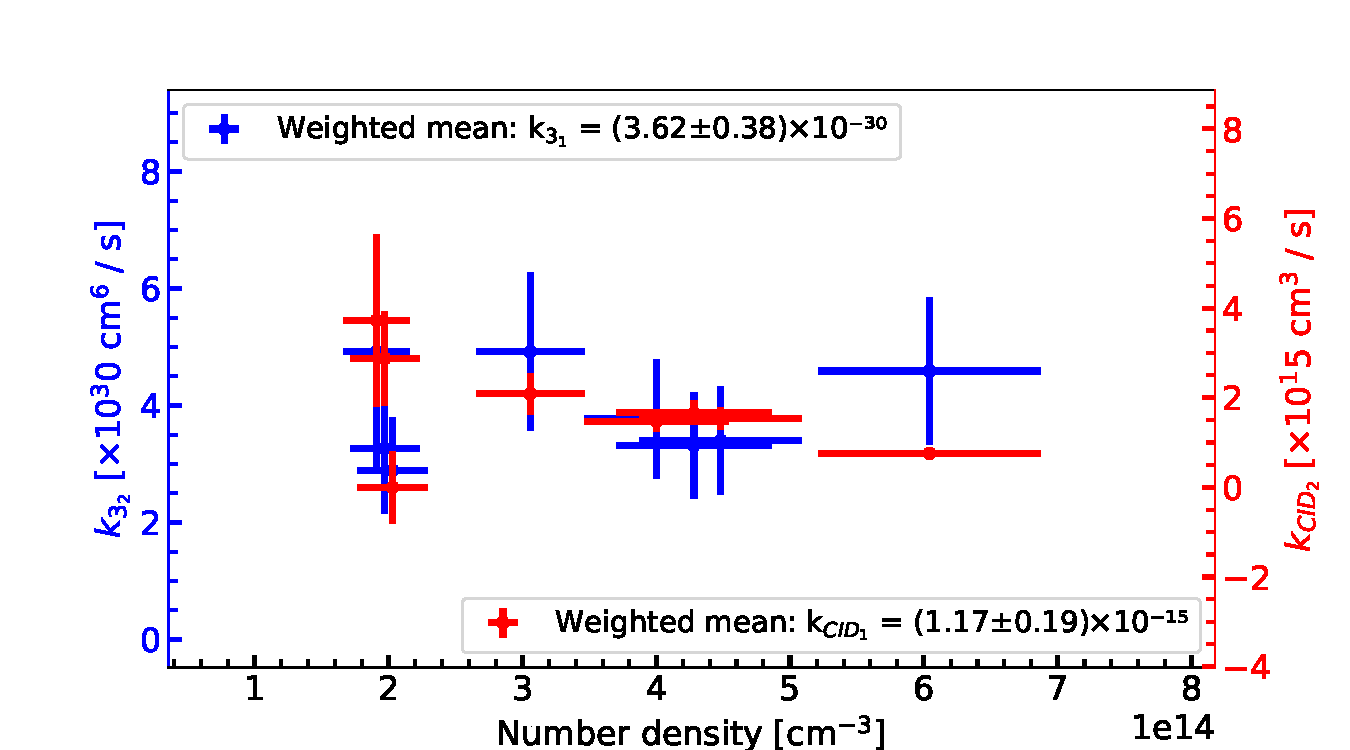
\includegraphics[width=1\textwidth]{figures/measurements/kinetics/rate-constants-higher-order/off_4.8K_k3_kCID_2_as_functionOfnHe.pdf}
        \caption{}
        
    \end{subfigure}
    \hfill
    \begin{subfigure}[b]{0.49\textwidth}
        \centering
        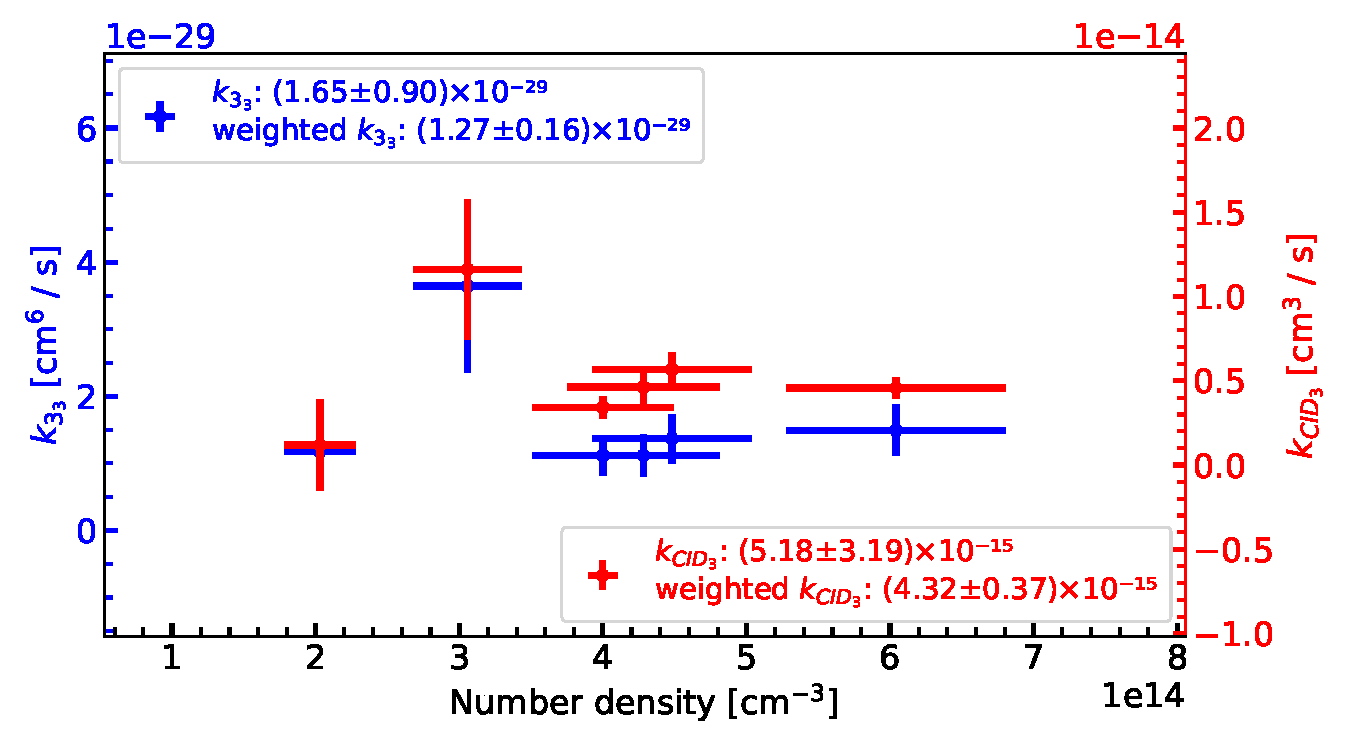
\includegraphics[width=1\textwidth]{figures/measurements/kinetics/rate-constants-higher-order/off_4.8K_k3_kCID_3_as_functionOfnHe.pdf}
        \caption{}
        
    \end{subfigure}
    
    \begin{subfigure}[b]{0.49\textwidth}
        \centering
        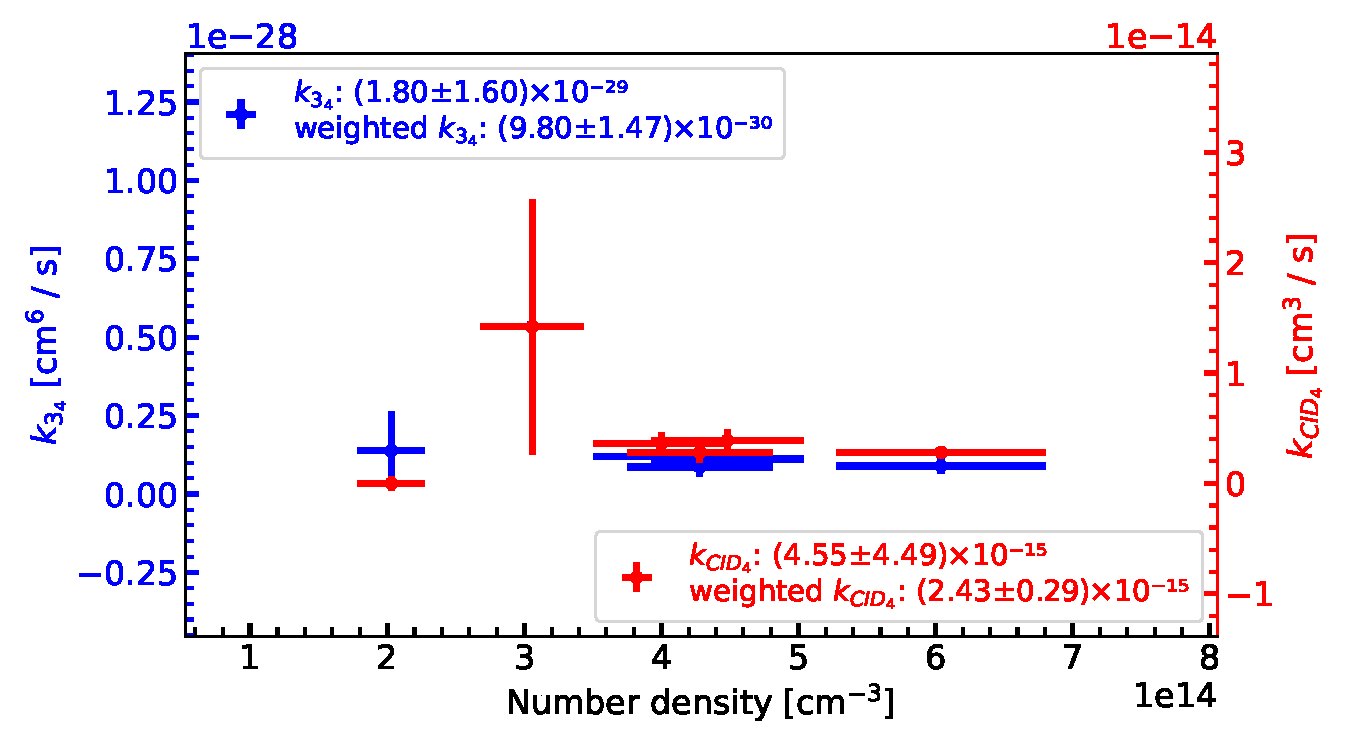
\includegraphics[width=1\textwidth]{figures/measurements/kinetics/rate-constants-higher-order/off_4.8K_k3_kCID_4_as_functionOfnHe.pdf}
        \caption{}
        
    \end{subfigure}
    \hfill
    \begin{subfigure}[b]{0.49\textwidth}
        \centering
        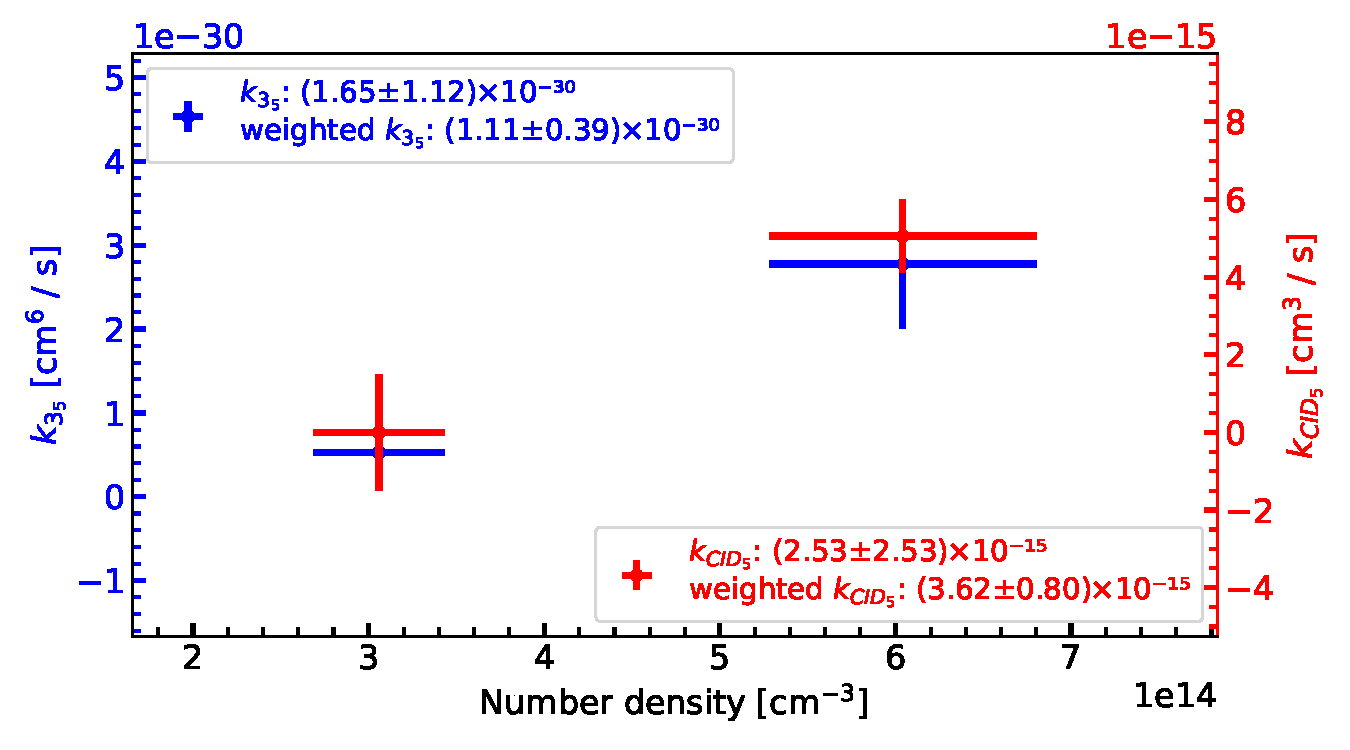
\includegraphics[width=1\textwidth]{figures/measurements/kinetics/rate-constants-higher-order/off_4.8K_k3_kCID_5_as_functionOfnHe.pdf}
        \caption{}
        
    \end{subfigure}
    
    \caption{The numerically derived formation and dissociation rate constants for higher order of complexes $(n>1)$ plotted as a function of number density at 4.8(3) K temperature.}
    \label{fig:rate-constants-higher-order}

\end{figure}

Figure \ref{fig:off:rate-constants} and \ref{fig:rate-constants-higher-order}
show the derived ternary association rate constants ($k_3$) at a nominal trap
temperature of 4.8(3) K using equation
\ref{eqn:rate-theory:k*-further-simplified}. Each data point results from a
single kinetics scan (as shown in Figure \ref{fig:fit:rate-constants}) at a
given number density. Since the rate constants are defined to be independent
(only when $k_3[He] >> k_r$) of number density, one can compute a weighted mean
value as reported in Table \ref{tab:k3:rate-constants} and
\ref{tab:kCID:rate-constants}. It should be noted that if the trap loss channel
is not included (see Section \ref{subsec:rate-loss-channels}), then the
formation rate ($k_3$) does not vary within the given error bar, but the
dissociation rate ($k_{CID}$) increases by $20-25\%$. This is also evidently
seen in Table \ref{tab:k3:rate-constants} and
\ref{tab:kCID:rate-constants}, i.e., the previously reported values
\cite{Brunken2017} for $k_{CID_n}$ significantly disagree due to
not considering the loss channels. However, the trap loss channel is
required to fit the total sum (indicated as a black line in Figure
\ref{fig:trap-and-m30-loss-channel-comparision}). Hence all the derived rate
constants include the trap loss and other loss channels as described in Section
\ref{subsec:rate-loss-channels}.